\section*{Introdução}

\paragraph{Objetivos.}

\begin{enumerate}
\item Entender os princípios (científicos) e conceitos por trás dos sistemas embarcados;
\item Obter uma experiência prática através da construção de projetos simples.
\item Ao final do curso, o aluno deverá:
\item Ser capaz de projetar sistemas embarcados efetuando a integração de componentes;
\item Analisar e desenvolver aplicações com os requisitos necessários para sistemas embarcados.
\end{enumerate}

\paragraph{Tópicos.}

\begin{enumerate}
\item Arquitetura de processadores para sistemas embarcados;
\item Funções básicas de microcontroladores;
\item Principais componentes: temporizadores, interrupções, porta serial (síncrona e assíncrona);
\item Programação de microcontroladores e placas de circuito;
\item Interação com dispositivos;
\item Interface com sensores e periféricos;
\item Princípios de sistemas de tempo real;
\item Aplicações e projetos de sistemas embarcados: microcontrolador 8051, Arduino. 
\end{enumerate}

\end{document}

\paragraph{Especificidade.}

\begin{enumerate}

	\item Computação geral: smartphones, tablets;
	\item Controle de sistemas: controladores de ambiente, velocidade;
	\item Processamento de sinais:radar, imagens de dispositivos médicos;
	\item Comunicação e rede: sistemas de telefonia, wireless, roteamento.
\end{enumerate}

\paragraph{Arquitetura.}

\begin{center}
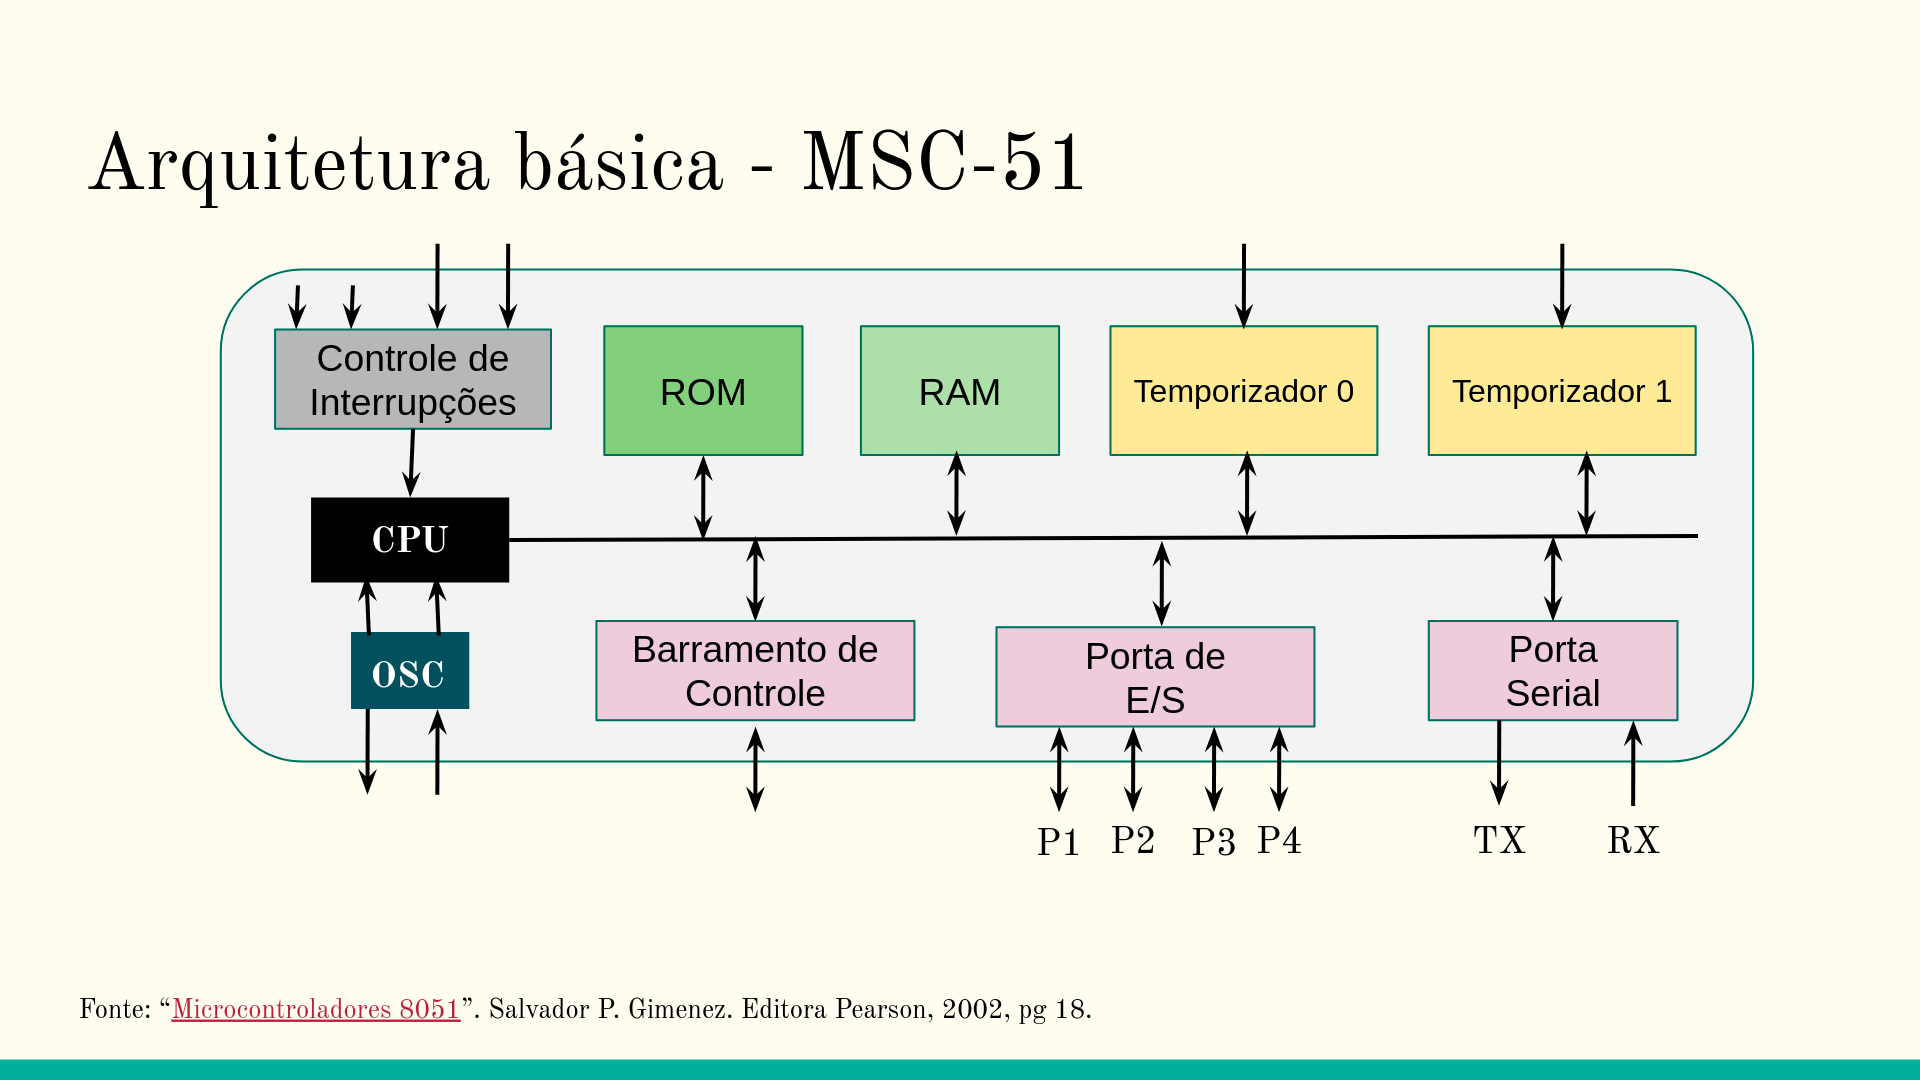
\includegraphics[scale=.5]{img/msc51_arch.png}
\end{center}

